\documentclass{article}
\usepackage[utf8]{inputenc}
\usepackage{xcolor}
\usepackage{tikz}
\usetikzlibrary{arrows.meta}

\begin{document}

\begin{figure}[h]
    \centering
    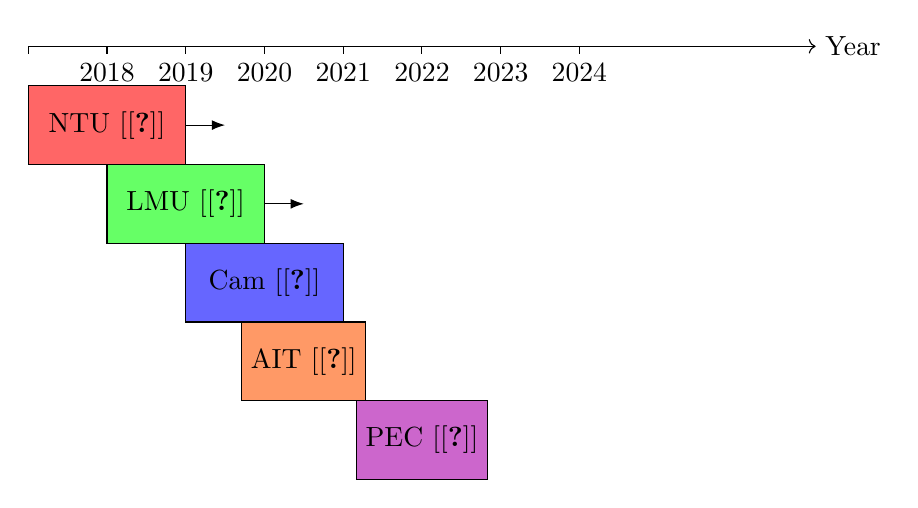
\begin{tikzpicture}[node distance = 1cm, auto]
        % Define colors for each block
        \definecolor{redColor}{RGB}{255, 102, 102}
        \definecolor{greenColor}{RGB}{102, 255, 102}
        \definecolor{blueColor}{RGB}{102, 102, 255}
        \definecolor{orangeColor}{RGB}{255, 153, 102}
        \definecolor{purpleColor}{RGB}{204, 102, 204}

        % Draw the timeline axis
        \draw[->] (0,0) -- (10,0) node[right] {Year};
        \draw (0,0) -- (0,-0.1);
        \foreach \x/\y in {1/2018, 2/2019, 3/2020, 4/2021, 5/2022, 6/2023, 7/2024} {
            \draw (\x*1,0) -- (\x*1,-0.1) node[below] {\y};
        }

        % Define nodes for each block
        \node[draw, fill=redColor, minimum width=2cm, minimum height=1cm] at (1, -1) (NTU) {NTU [\cite{ntu}]};
        \node[draw, fill=greenColor, minimum width=2cm, minimum height=1cm] at (2, -2) (LMU) {LMU [\cite{lmu}]};
        \node[draw, fill=blueColor, minimum width=2cm, minimum height=1cm] at (3, -3) (Cam) {Cam [\cite{cam}]};
        \node[draw, fill=orangeColor, minimum width=1.5cm, minimum height=1cm] at (3.5, -4) (AIT) {AIT [\cite{ait}]};
        \node[draw, fill=purpleColor, minimum width=1.5cm, minimum height=1cm] at (5, -5) (PEC) {PEC [\cite{pec}]};

        % Draw arrows between blocks
        \draw[-Latex] (NTU.east) -- (2.5, -1);
        \draw[-Latex] (LMU.east) -- (3.5, -2);
    \end{tikzpicture}
    \caption{Timeline of research activities by leading groups from 2018 to 2023, illustrating the dynamic landscape of contributions in the fields of digital forensics, disinformation detection, and generative AI. Each colored box represents a significant milestone or publication by the respective research group.}
    \label{fig:timeline}
\end{figure}

\begin{thebibliography}{9}
\bibitem{ntu} NTU Research Group, "NTU Publication."
\bibitem{lmu} LMU Research Team, "LMU Publication."
\bibitem{cam} Cam University Group, "Cam University Publication."
\bibitem{ait} AIT Institute, "AIT Publication."
\bibitem{pec} PEC Center, "PEC Publication."
\end{thebibliography}

\end{document}